\documentclass{article}
\usepackage{tabularx}
\usepackage{amsmath}
\usepackage{graphicx}
\usepackage[top = 2cm, bottom = 2cm, right = 2cm, left = 2cm]{geometry}
\usepackage{cite}
\usepackage[final]{hyperref}
\usepackage{listings}
\hypersetup{
	colorlinks=true,
	linkcolor=blue,
	citecolor=blue,
	filecolor=magenta,
	urlcolor=blue         
}

\begin{document}

\title{Practicle 7\\POO with CUDA}
\date{13/02/19}
\maketitle

\begin{abstract}
	
\end{abstract}

\section{Allocate memory from the device}
With CUDA, we have the ability to allocate memory from a kernel or a device function. To test that, we'll create spheres in a kernel. Create a kernel called generateSpheres.
\begin{lstlisting}
	__global__ void createWorld(Sphere** spheres) {}
\end{lstlisting}
On the host side we just have to create an array of pointer on sphere and allocate them on the device memory.
\begin{lstlisting}
	Sphere** spheres;
	cudaMalloc((void **)&spheres, nbSpheres*sizeof(Sphere*));
\end{lstlisting}

On our kernel we can now allocate memory on the device memory using the 'new' keyword.
\begin{lstlisting}
	spheres[0] = new Sphere(Vector3(0.f, -100.5f, -1.f), 100.f);
	spheres[1] = new Sphere(Vector3(0.f, 0.f, -3.f), 0.5f);
\end{lstlisting}

Spheres have to be generated only once. So, we call the kernel with one thread per blocks and one block per grids. CUDA will send 32 threads for this computation. CUDA should disable out of bounds threads, but it may a good option to scope the sphere generation.
\begin{lstlisting}
	if (threadIdx.x==0 && blockIdx.x==0) {
		spheres[0] = new Sphere(Vector3(0.f, -100.5f, -1.f), 100.f);
		spheres[1] = new Sphere(Vector3(0.f, 0.f, -3.f), 0.5f);
	}
\end{lstlisting}

Before calling the cudaFree on spheres, we must free the memory allocate in the device memory. In the same way, create a kernel called freeSpheresGenerated and use the delete keyword (as C++) to free the sphere from the kernel.

\section{Material}
We see on the chapter before that materials are basically just a scatter function. We defined the diffuse material and now we focus the metal and dielectric material. Create a class material with a virtual pure scatter function. His parameters are the current ray, the hit structure and the random states. By reference pass the Vector3 attenuation and rayScattered to compute. The return of this function is a boolean to check the validity of the scattered ray.
\begin{lstlisting}
	__device__ virtual bool scatter(
		const Ray& ray,
		const HitInformation& hit,
		Vector3& attenuation,
		Ray& rayScattered,
		curandState* states) const = 0;
\end{lstlisting}

Each spheres in our world will have a material. So, we need to add a pointer to material in the sphere class and in the HitInformation.

\begin{lstlisting}
	Material* material_;
\end{lstlisting}

It's very rare that two spheres share the same color and material properties. So, we can assume we have one material per sphere. The material\_ member store the material and get the ownership of the pointer. Because of that, we must free the material on the freeSpheresGenerated before the delete of the sphere.\\
And when a ray hit a sphere, we can add the material information into the hit.

\begin{lstlisting}
	hit.material_ = sphere.getMaterial();
\end{lstlisting}

\subsection{Diffuse material}
Create a class DiffuseMaterial that extends Material.
\begin{lstlisting}
	class DiffuseMaterial : public Material
\end{lstlisting}

The overrode scatter function should return true. The computation of the scattered ray and the absorption isn't changed.

\begin{lstlisting}
	Vector3 target = hit.intersection_ + hit.normal_ + randomSphereUnitVector(states);
	rayScattered = Ray(hit.intersection_, (target-hit.intersection_));
	attenuation = sphereColor_;
	return true;
\end{lstlisting}

On your rendering function you just need to call the scatter function stored in the hit information.
\begin{lstlisting}
	//...
	if (hit.hit_) {
		Ray scattered;
		Vector3 attenuation;
		if (hit.material_->scatter(r, hit, attenuation, scattered, states)) {
			r = scattered;
			cur_attenuation *= attenuation;
		} else {
			return Vector3(0.f, 0.f, 0.f);
		}
	}
	//...
\end{lstlisting}

We can now add the material to our sphere during the world generation.
\begin{lstlisting}
	Vector3 sphereColor = Vector3(0.7f, 0.7f, 0.7f);
	spheres[0] = new Sphere(Vector3(0.f, -100.5f, -1.f), 100.f,
		new DiffuseMaterial(sphereColor));
\end{lstlisting}

\subsection{Metal material}
When a ray hit a metal it is reflected. So, we just need to compute the symmetric ray of the ray direction using the normal. Create a device function reflect.
\begin{lstlisting}
	__device__ Vector3 reflect(const Vector3& d, const Vector3& n) {
		return d-2.f*dot(d, n)*n;
	}
\end{lstlisting}
Perfect metal reflect the input ray. If we want a more realistic result we can add a random reflection drove by a fuzz parameter. With this extra parameter we need to discard scattered ray inside the sphere.

\begin{lstlisting}
	Vector3 reflected = reflect(ray.getDirection(), hit.normal_);
	rayScattered = Ray(hit.intersection_, 
		reflected + fuzz_*randomSphereUnitVector(states));
	attenuation = color_;
	return (dot(rayScattered.getDirection(), hit.normal_) > 0.f);
\end{lstlisting}

\begin{figure}[h]
	\centering
	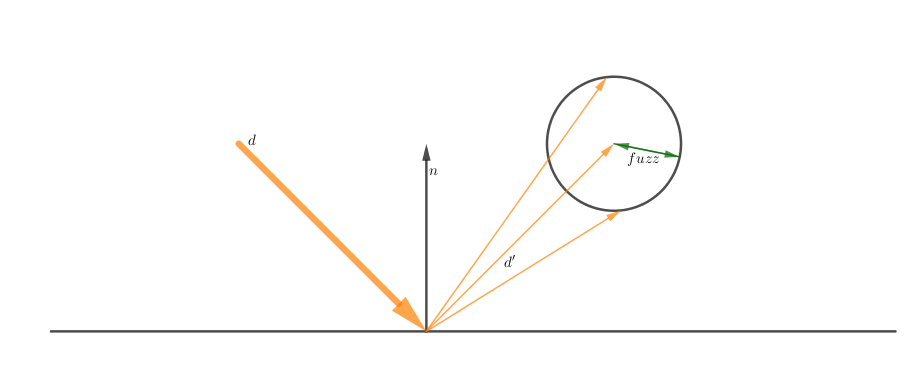
\includegraphics[scale=0.7]{figures/metal.png}
	\caption{Metal material}
\end{figure}

\begin{figure}[h]
	\centering
	\includegraphics[scale=0.2]{figures/metalFuzz.png}
	\caption{Fuzz parameter}
\end{figure}

\subsection{Dialectric material}
Rays hit dielectric material can be both reflected or refracted. The ray can go through the object, so every scattered ray are valid. This function can return always true. The Index Of Refraction (IOR) is the only class member we need. If you want to create a water material you can choose 1.33.

\subsubsection{Transition}
When a ray hit the surface of a dielectric object it can go from the outside or the inside of the sphere. A positive dot product between the normal and the ray direction mean the ray came from the outside. For the refraction we need the normal of the opposite material.
\begin{lstlisting}
	bool fromOutside = dot(ray.getDirection(), hit.normal_)>0;
	if (fromOutside) {
		normal = -hit.normal_;
	} else {
		normal = hit.normal_;
	}
\end{lstlisting}

\subsubsection{Refraction}
We assume outside spheres is vacuum (IOR 1). We can simplify the Snell's law and the ratio of sines become $\frac{sin\theta_2}{sin\theta_1} = \frac{n_2}{n_1}$.
\begin{lstlisting}
	if (fromOutside) {
		ratio = ior_/1.f;
	} else {
		ratio = 1.f/ior_;
	}
\end{lstlisting}
Create a device function to compute the refraction.
\begin{lstlisting}
__device__ 
bool refract(const Vector3& v, const Vector3& n, float ratio, Vector3& refracted) {
	float dt = dot(v, n);
	float discriminant = 1.f-ratio*ratio*(1.f-dt*dt);
	if (discriminant>0) {
		refracted = ratio*(v-n*dt)-n*sqrt(discriminant);
		return true;
	} else {
		return false;
	}
}
\end{lstlisting}
If the refraction failed, the probability of the reflection becomes 1.

\subsubsection{Fresnel coefficients}
The Fresnel equations describe the reflection and refraction of an electromagnetic radiation. The Fresnel's coefficient describe the reflected probability in the case of the refraction is possible. We can use the Schlick's approximation $R(\theta) = R_0 + (1-R_0)(1-cos\theta)^5$ with $R_0 = (\frac{n_1 - n_2}{n_1 + n_2})^2$.
\begin{lstlisting}
	if (fromOutside) {
		cosTheta = ior_*dot(ray.getDirection(), hit.normal_);
	} else {
		cosTheta = -dot(ray.getDirection(), hit.normal_);
	}
	float r0 = (1.f-ior_)/(1.f+ior_);
	r0 = r0*r0;
	float reflectProbability = r0+(1.f-r0)*pow((1.f-cosTheta), 5.f);
\end{lstlisting}

\newpage
\subsubsection{Dialectric scatter function}
\begin{lstlisting}
	Vector3 normal;
	float ratio;
	float cosTheta;
	attenuation = Vector3(1.f, 1.f, 1.f);
	if (dot(ray.getDirection(), hit.normal_)>0) {
		normal = -hit.normal_;
		ratio = ior_;
		cosTheta = ior_*dot(ray.getDirection(), hit.normal_);
	} else {
		normal = hit.normal_;
		ratio = 1.f/ior_;
		cosTheta = -dot(ray.getDirection(), hit.normal_);
	}
	Vector3 refracted;
	float reflectProbability;
	if (refract(ray.getDirection(), normal, ratio, refracted)) {
		reflectProbability = schlick(cosTheta, ior_);
	} else {
		rayScattered = Ray(
			hit.intersection_,
			reflect(ray.getDirection(), hit.normal_));
		return true;
	}
	if (curand_uniform(states)<reflectProbability) {
		rayScattered = Ray(
			hit.intersection_,
			reflect(ray.getDirection(), hit.normal_));
	} else {
		rayScattered = Ray(hit.intersection_, refracted);
	}
	return true;
\end{lstlisting}

\newpage
\section{Result}
\begin{figure}[h]
	\centering
	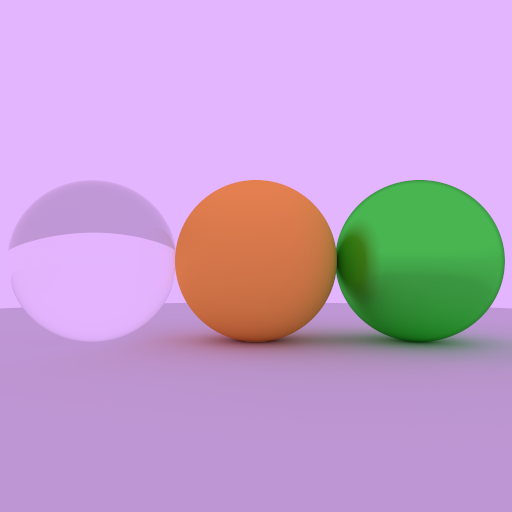
\includegraphics[scale=0.99]{figures/final.png}
	\caption{Final render}
\end{figure}

\end{document}